% Generated by pysimcount.pfchilds -- do not edit; regenerate instead.
% figure: main-cnot-all-formulas -- Every formula, X-Y-Z grouping, cnot gates vs n (cf. Childs et al. 2018 Fig. 3 right)
% source: ../np-main/aggregate.json + ../np-main-n9/seed{seed}, ../np-main-n11/seed{seed} (seeds [1, 2, 3, 4, 5, 6, 7, 8, 9, 10]); run commits: 01d3c275ceae2840002bd1aaea68f59b987c4975, e42ff29056ad9ea7fc7c9899fab334903e42e3e3
% metric=cnot kind=xyz merged (cz, simcount template)
% measured n: mean over seeds of the run's totals; bars min..max over seeds
% r from power-law fit to mean measured r (n = 5--11); r = ceil(a n^b); bars = min..max of per-seed fits
% per-step counts exactly affine in n (checked on n = [10, 20, 40], direct build at n = [100])
% shown: suzuki4, suzuki6, mo-q6, mo-q14, bm-q10, mo-o8-q21, morales-y8m10, morales-m8
% removed (see main-cnot-all-formulas-ranking.md): lie-trotter, suzuki2, suzuki8
% figure made at git_commit=e42ff29056ad9ea7fc7c9899fab334903e42e3e3 git_dirty=True
% WARNING: made from uncommitted code; the commit above does not reproduce it.
% derived: main-cnot-all-formulas.tex restyled by pysimcount.figuniform: extrapolated points (r from power-law fit) drawn in their series' measured style, style-key legend entries removed; extrapolated n = [13, 20, 30, 50, 70, 100, 200, 300, 500]; source_sha256=d08ff822c5bf1fad500b9ec916dfdb169761fa795678e567d52587afb36bc628
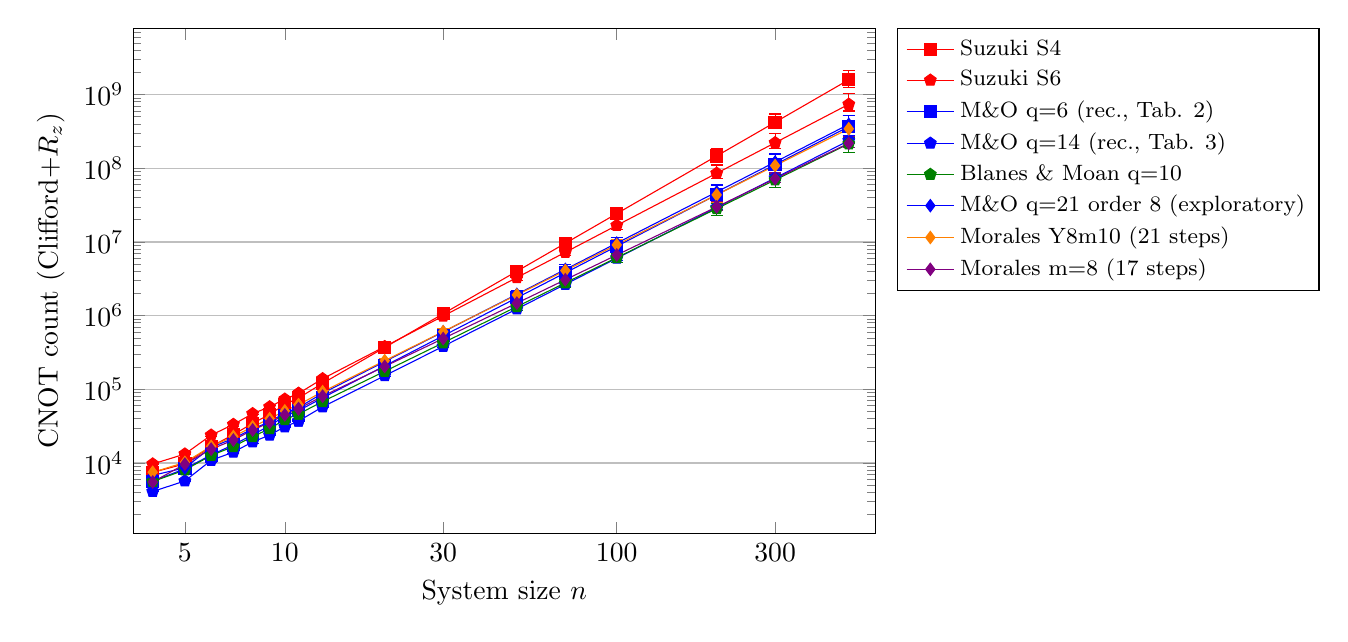
\begin{tikzpicture}
  \begin{loglogaxis}[
    width=11cm, height=8cm,
    xlabel={System size $n$},
    ylabel={CNOT count (Clifford+$R_z$)},
    xtick={5,10,30,100,300}, xticklabels={5,10,30,100,300},
    xmin=3.5, xmax=600,
    ymajorgrids=true,
    legend pos=outer north east,
    legend cell align=left,
    legend style={font=\footnotesize},
  ]
    % suzuki4: measured n, mean over seeds, bars min..max over seeds
    \addplot[red, solid, mark=square*, mark size=2.2pt, mark options={solid, fill=red}, error bars/.cd, y dir=both, y explicit, error bar style={solid}] coordinates {
      (4,7459.2) += (0,100.8) -= (0,67.2)
      (5,9744) += (0,336) -= (0,294)
      (6,16707.6) += (0,1184.4) -= (0,831.6)
      (7,24284.4) += (0,1881.6) -= (0,1646.4)
      (8,34540.8) += (0,1411.2) -= (0,1276.8)
      (9,45549) += (0,2079) -= (0,2457)
      (10,62412) += (0,4788) -= (0,2352)
      (11,76230) += (0,3234) -= (0,1848)
    };
    \addlegendentry{Suzuki S4}
    % suzuki4: extrapolated, r = ceil(3.65267 n^1.59931), per step = 42 n + 0; bars min..max of per-seed fits
    \addplot[red, solid, mark=square*, mark size=2.2pt, mark options={solid, fill=red}, forget plot, error bars/.cd, y dir=both, y explicit, error bar style={solid}] coordinates {
      (11,76230)
      (13,120666) += (0,5460) -= (0,3822)
      (20,369600) += (0,27720) -= (0,20160)
      (30,1.06092e+06) += (0,109620) -= (0,80640)
      (50,4.0005e+06) += (0,575400) -= (0,403200)
      (70,9.59322e+06) += (0,1.63758e+06) -= (0,1.12308e+06)
      (100,2.42382e+07) += (0,4.8552e+06) -= (0,3.2424e+06)
      (200,1.46882e+08) += (0,3.81108e+07) -= (0,2.43096e+07)
      (300,4.21382e+08) += (0,1.24501e+08) -= (0,7.73136e+07)
      (500,1.58972e+09) += (0,5.44026e+08) -= (0,3.26886e+08)
    };
    % suzuki6: measured n, mean over seeds, bars min..max over seeds
    \addplot[red, solid, mark=pentagon*, mark size=2.2pt, mark options={solid, fill=red}, error bars/.cd, y dir=both, y explicit, error bar style={solid}] coordinates {
      (4,9696) += (0,0) -= (0,0)
      (5,13231) += (0,909) -= (0,101)
      (6,23876.4) += (0,1575.6) -= (0,848.4)
      (7,33370.4) += (0,1979.6) -= (0,2262.4)
      (8,46702.4) += (0,1777.6) -= (0,1454.4)
      (9,57812.4) += (0,2181.6) -= (0,3272.4)
      (10,73528) += (0,5252) -= (0,2828)
      (11,87991.2) += (0,3110.8) -= (0,1333.2)
    };
    \addlegendentry{Suzuki S6}
    % suzuki6: extrapolated, r = ceil(1.63295 n^1.35284), per step = 202 n + 0; bars min..max of per-seed fits
    \addplot[red, solid, mark=pentagon*, mark size=2.2pt, mark options={solid, fill=red}, forget plot, error bars/.cd, y dir=both, y explicit, error bar style={solid}] coordinates {
      (11,87991.2)
      (13,139178) += (0,7878) -= (0,2626)
      (20,379760) += (0,32320) -= (0,12120)
      (30,987780) += (0,115140) -= (0,54540)
      (50,3.2825e+06) += (0,535300) -= (0,272700)
      (70,7.23968e+06) += (0,1.39986e+06) -= (0,721140)
      (100,1.6766e+07) += (0,3.7774e+06) -= (0,1.9594e+06)
      (200,8.55672e+07) += (0,2.50884e+07) -= (0,1.2726e+07)
      (300,2.2216e+08) += (0,7.41138e+07) -= (0,3.71478e+07)
      (500,7.38916e+08) += (0,2.8583e+08) -= (0,1.40087e+08)
    };
    % mo-q6: measured n, mean over seeds, bars min..max over seeds
    \addplot[blue, solid, mark=square*, mark size=2.2pt, mark options={solid, fill=blue}, error bars/.cd, y dir=both, y explicit, error bar style={solid}] coordinates {
      (4,5660) += (0,340) -= (0,660)
      (5,8350) += (0,400) -= (0,850)
      (6,12870) += (0,330) -= (0,570)
      (7,17675) += (0,875) -= (0,1225)
      (8,24160) += (0,2240) -= (0,1360)
      (9,32085) += (0,1665) -= (0,2385)
      (10,43300) += (0,1700) -= (0,2800)
      (11,51260) += (0,5390) -= (0,4510)
    };
    \addlegendentry{M\&O q=6 (rec., Tab. 2)}
    % mo-q6: extrapolated, r = ceil(3.93927 n^1.32338), per step = 50 n + 0; bars min..max of per-seed fits
    \addplot[blue, solid, mark=square*, mark size=2.2pt, mark options={solid, fill=blue}, forget plot, error bars/.cd, y dir=both, y explicit, error bar style={solid}] coordinates {
      (11,51260)
      (13,76700) += (0,4550) -= (0,3250)
      (20,208000) += (0,21000) -= (0,13000)
      (30,532500) += (0,73500) -= (0,48000)
      (50,1.745e+06) += (0,322500) -= (0,212500)
      (70,3.815e+06) += (0,822500) -= (0,539000)
      (100,8.735e+06) += (0,2.19e+06) -= (0,1.415e+06)
      (200,4.371e+07) += (0,1.402e+07) -= (0,8.78e+06)
      (300,1.12125e+08) += (0,4.077e+07) -= (0,2.4975e+07)
      (500,3.67375e+08) += (0,1.542e+08) -= (0,9.1575e+07)
    };
    % mo-q14: measured n, mean over seeds, bars min..max over seeds
    \addplot[blue, solid, mark=pentagon*, mark size=2.2pt, mark options={solid, fill=blue}, error bars/.cd, y dir=both, y explicit, error bar style={solid}] coordinates {
      (4,4104) += (0,0) -= (0,0)
      (5,5700) += (0,0) -= (0,0)
      (6,10875.6) += (0,68.4) -= (0,615.6)
      (7,14044.8) += (0,319.2) -= (0,478.8)
      (8,19334.4) += (0,729.6) -= (0,1094.4)
      (9,23905.8) += (0,718.2) -= (0,307.8)
      (10,31008) += (0,912) -= (0,228)
      (11,37118.4) += (0,501.6) -= (0,752.4)
    };
    \addlegendentry{M\&O q=14 (rec., Tab. 3)}
    % mo-q14: extrapolated, r = ceil(1.412 n^1.28559), per step = 114 n + 0; bars min..max of per-seed fits
    \addplot[blue, solid, mark=pentagon*, mark size=2.2pt, mark options={solid, fill=blue}, forget plot, error bars/.cd, y dir=both, y explicit, error bar style={solid}] coordinates {
      (11,37118.4)
      (13,57798) += (0,0) -= (0,1482)
      (20,152760) += (0,4560) -= (0,4560)
      (30,383040) += (0,20520) -= (0,13680)
      (50,1.2312e+06) += (0,91200) -= (0,57000)
      (70,2.65734e+06) += (0,239400) -= (0,143640)
      (100,6.0078e+06) += (0,638400) -= (0,364800)
      (200,2.92524e+07) += (0,4.1268e+06) -= (0,2.1204e+06)
      (300,7.3872e+07) += (0,1.197e+07) -= (0,5.9166e+06)
      (500,2.37462e+08) += (0,4.4574e+07) -= (0,2.1261e+07)
    };
    % bm-q10: measured n, mean over seeds, bars min..max over seeds
    \addplot[green!50!black, solid, mark=pentagon*, mark size=2.2pt, mark options={solid, fill=green!50!black}, error bars/.cd, y dir=both, y explicit, error bar style={solid}] coordinates {
      (4,5608.8) += (0,295.2) -= (0,32.8)
      (5,8036) += (0,164) -= (0,246)
      (6,12644.4) += (0,147.6) -= (0,344.4)
      (7,16703.4) += (0,516.6) -= (0,631.4)
      (8,22828.8) += (0,1443.2) -= (0,1180.8)
      (9,29151) += (0,1107) -= (0,1845)
      (10,38868) += (0,492) -= (0,1148)
      (11,46182.4) += (0,2525.6) -= (0,1984.4)
    };
    \addlegendentry{Blanes \& Moan q=10}
    % bm-q10: extrapolated, r = ceil(2.82314 n^1.2111), per step = 82 n + 0; bars min..max of per-seed fits
    \addplot[green!50!black, solid, mark=pentagon*, mark size=2.2pt, mark options={solid, fill=green!50!black}, forget plot, error bars/.cd, y dir=both, y explicit, error bar style={solid}] coordinates {
      (11,46182.4)
      (13,68224) += (0,1066) -= (0,2132)
      (20,175480) += (0,6560) -= (0,9840)
      (30,428040) += (0,27060) -= (0,34440)
      (50,1.3243e+06) += (0,123000) -= (0,143500)
      (70,2.7839e+06) += (0,309960) -= (0,355880)
      (100,6.1254e+06) += (0,811800) -= (0,902000)
      (200,2.83392e+07) += (0,4.9856e+06) -= (0,5.1824e+06)
      (300,6.94704e+07) += (0,1.39482e+07) -= (0,1.41204e+07)
      (500,2.14922e+08) += (0,5.0184e+07) -= (0,4.9036e+07)
    };
    % mo-o8-q21: measured n, mean over seeds, bars min..max over seeds
    \addplot[blue, solid, mark=diamond*, mark size=2.2pt, mark options={solid, fill=blue}, error bars/.cd, y dir=both, y explicit, error bar style={solid}] coordinates {
      (4,6800) += (0,0) -= (0,0)
      (5,8585) += (0,765) -= (0,85)
      (6,16320) += (0,1020) -= (0,1020)
      (7,21539) += (0,1071) -= (0,1309)
      (8,28968) += (0,952) -= (0,1768)
      (9,36261) += (0,459) -= (0,1071)
      (10,47770) += (0,3230) -= (0,1870)
      (11,56661) += (0,1309) -= (0,561)
    };
    \addlegendentry{M\&O q=21 order 8 (exploratory)}
    % mo-o8-q21: extrapolated, r = ceil(1.3736 n^1.30758), per step = 170 n + 0; bars min..max of per-seed fits
    \addplot[blue, solid, mark=diamond*, mark size=2.2pt, mark options={solid, fill=blue}, forget plot, error bars/.cd, y dir=both, y explicit, error bar style={solid}] coordinates {
      (11,56661)
      (13,88400) += (0,2210) -= (0,2210)
      (20,238000) += (0,13600) -= (0,10200)
      (30,601800) += (0,51000) -= (0,35700)
      (50,1.9465e+06) += (0,255000) -= (0,170000)
      (70,4.2364e+06) += (0,666400) -= (0,452200)
      (100,9.639e+06) += (0,1.819e+06) -= (0,1.224e+06)
      (200,4.7668e+07) += (0,1.19e+07) -= (0,7.752e+06)
      (300,1.21482e+08) += (0,3.4833e+07) -= (0,2.2185e+07)
      (500,3.94825e+08) += (0,1.3226e+08) -= (0,8.211e+07)
    };
    % morales-y8m10: measured n, mean over seeds, bars min..max over seeds
    \addplot[orange, solid, mark=diamond*, mark size=2.2pt, mark options={solid, fill=orange}, error bars/.cd, y dir=both, y explicit, error bar style={solid}] coordinates {
      (4,7480) += (0,0) -= (0,0)
      (5,10200) += (0,0) -= (0,0)
      (6,16830) += (0,510) -= (0,510)
      (7,22848) += (0,952) -= (0,238)
      (8,31008) += (0,1632) -= (0,1088)
      (9,39933) += (0,1377) -= (0,1683)
      (10,51000) += (0,3400) -= (0,1700)
      (11,61710) += (0,1870) -= (0,1870)
    };
    \addlegendentry{Morales Y8m10 (21 steps)}
    % morales-y8m10: extrapolated, r = ceil(1.66328 n^1.25438), per step = 170 n + 0; bars min..max of per-seed fits
    \addplot[orange, solid, mark=diamond*, mark size=2.2pt, mark options={solid, fill=orange}, forget plot, error bars/.cd, y dir=both, y explicit, error bar style={solid}] coordinates {
      (11,61710)
      (13,92820) += (0,2210) -= (0,4420)
      (20,244800) += (0,13600) -= (0,17000)
      (30,606900) += (0,56100) -= (0,56100)
      (50,1.9125e+06) += (0,238000) -= (0,238000)
      (70,4.0936e+06) += (0,595000) -= (0,595000)
      (100,9.129e+06) += (0,1.581e+06) -= (0,1.513e+06)
      (200,4.3554e+07) += (0,9.758e+06) -= (0,8.908e+06)
      (300,1.0863e+08) += (0,2.7693e+07) -= (0,2.4582e+07)
      (500,3.4357e+08) += (0,1.0132e+08) -= (0,8.6955e+07)
    };
    % morales-m8: measured n, mean over seeds, bars min..max over seeds
    \addplot[violet, solid, mark=diamond*, mark size=2.2pt, mark options={solid, fill=violet}, error bars/.cd, y dir=both, y explicit, error bar style={solid}] coordinates {
      (4,5520) += (0,0) -= (0,0)
      (5,9660) += (0,0) -= (0,0)
      (6,15400.8) += (0,331.2) -= (0,496.8)
      (7,20479.2) += (0,772.8) -= (0,193.2)
      (8,28041.6) += (0,1766.4) -= (0,441.6)
      (9,35397) += (0,621) -= (0,621)
      (10,44988) += (0,1932) -= (0,828)
      (11,54496.2) += (0,1669.8) -= (0,1366.2)
    };
    \addlegendentry{Morales m=8 (17 steps)}
    % morales-m8: extrapolated, r = ceil(2.19247 n^1.17079), per step = 138 n + 0; bars min..max of per-seed fits
    \addplot[violet, solid, mark=diamond*, mark size=2.2pt, mark options={solid, fill=violet}, forget plot, error bars/.cd, y dir=both, y explicit, error bar style={solid}] coordinates {
      (11,54496.2)
      (13,80730) += (0,1794) -= (0,1794)
      (20,204240) += (0,8280) -= (0,8280)
      (30,488520) += (0,33120) -= (0,24840)
      (50,1.4766e+06) += (0,144900) -= (0,96600)
      (70,3.07188e+06) += (0,338100) -= (0,231840)
      (100,6.6516e+06) += (0,883200) -= (0,579600)
      (200,2.99184e+07) += (0,5.1336e+06) -= (0,3.2016e+06)
      (300,7.21602e+07) += (0,1.39932e+07) -= (0,8.6112e+06)
      (500,2.18661e+08) += (0,4.899e+07) -= (0,2.9325e+07)
    };
  \end{loglogaxis}
\end{tikzpicture}
